\section{Adaptive Komponente in Hadoop}
\label{sec:inriaSetting}

Eine normale Hadoop"=Installation besitzt keine adaptive Komponente, sondern rein statische Einstellungen.
Um damit Hadoop zu optimieren, müssen die Einstellungen daher immer manuell auf den jeweils benötigten Anwendungstyp angepasst werden.
Dazu gibt es verschiedene Scheduler, den \emph{Fair Scheduler}, welcher alle Anwendungen ausführt und ihnen gleich viele Ressourcen zuteilt, und den \emph{Capacity Scheduler}.
Letzterer sorgt dafür, dass nur eine bestimmte Anzahl an Anwendungen pro Benutzter gleichzeitig ausgeführt wird und teilt ihnen so viele Ressourcen zu, wie benötigt werden bzw. der Benutzter nutzen darf.
Entwickelt wurde der Capacity Scheduler vor allem für Cluster, die von mehreren Organisationen gemeinsam verwendet werden und sicherstellen soll, dass jede Organisation eine Mindestmenge an Ressourcen zur Verfügung hat \cite{HadoopCapScheduler271}.
Für diesen Scheduler wurde in \cite{zhang2016} ein selbst"=adaptiver Ansatz vorgestellt, welcher im Folgenden genauer erläutert wird.

\subsection{\acs{MARP}"=Wert}
\label{sec:selfbalancingMarp}

Der Capacity Scheduler verschiedene Einstellungen, um ihn für das konkrete Cluster anzupassen.
So besteht \zB die Möglichkeit, den verfügbaren Speicher pro Anwendungs"=Container festzulegen oder wie viel Ressourcen durch \ac{AppMstr}"=Container beansprucht werden darf.
Vor allem letztere Einstellungsmöglichkeit namens \ac{MARP} ist sehr wichtig, wenn mehrere Anwendungen gleichzeitig ausgeführt werden sollen.
Der in der Konfiguration des Schedulers definierte \ac{MARP}"=Wert gibt an, wie viel Prozent des verfügbaren Speichers durch \ac{AppMstr}"=Container genutzt werden darf \cite{HadoopCapScheduler271}.
Der gesamte, für Anwendungen verfügbare Speicher wird durch den \ac{MARP}"=Wert in zwei Teile aufgeteilt.
Während der einen Teil des Speichers nur durch \ac{AppMstr}"=Container beansprucht werden darf, wird der andere Teil des Speichers durch alle anderen Anwendungs"=Container genutzt.
Wird durch den \ac{MARP}"=Wert der erste, für für \ac{AppMstr}"=reservierten Teil zu klein gehalten, können daher weniger \ac{AppMstr} allokiert werden und somit auch weniger Anwendungen gestartet werden (\emph{Loss of Jobs Parallelism}, LoJP).
Ist der \ac{MARP}"=Wert dagegen zu groß, wird der verfügbare Speicher zu entsprechend großen Teilen für mögliche \ac{AppMstr} reserviert.
Dadurch ist der Anteil des Speichers für Anwendungs"=Container entsprechend klein und es können dadurch weniger Container gestartet werden, um eine Anwendung auszuführen, womit sich die Ausführungsgeschwindigkeit der Anwendungen verringert (\emph{Loss of Job Throughput}, LoJT) \cite{zhang2016}:

\begin{figure}[h]
    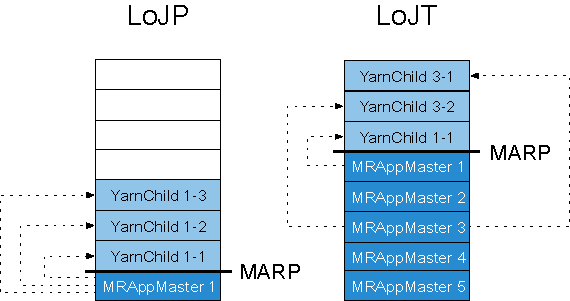
\includegraphics{./images/marpValue.pdf}
    \caption[LoJP und LoJT in Hadoop]
    {LoJP und LoJT in Hadoop (entnommen aus \cite{zhang2016}).
        Während beim LoJP sehr viel Speicher für Anwendungs"=Container ungenutzt bleibt, können beim LoJT nicht genügend Anwendungs"=Container allokiert werden, um die Anwendungen auszuführen.}
    \label{fig:marpValue}
\end{figure}

Damit bestimmt der \ac{MARP}"=Wert indirekt auch die maximale Anzahl an Anwendungen, die gleichzeitig ausgeführt werden können.
Da der \ac{MARP}"=Wert jedoch nicht während der Laufzeit dynamisch angepasst werden kann, haben \citeauthor{zhang2016} in \cite{zhang2016} einen Ansatz zur dynamischen Anpassung des \ac{MARP}"=Wertes zur Laufzeit von Hadoop vorgestellt.
Die entwickelte \textbf{Selfbalancing"=Komponente} passt den \ac{MARP}"=Wert abhängig von der Speicherauslastung der ausgeführten Anwendungen dynamisch zur Laufzeit an.
So wird der \ac{MARP}"=Wert verringert, wenn die Speicherauslastung sehr hoch ist, und erhöht, wenn die Speicherauslastung sehr niedrig ist.
Die Selfbalancing"=Komponente ermöglicht daher, dass immer die maximal mögliche Anzahl an Anwendungen ausgeführt werden kann.
Die Evaluation von \citeauthor{zhang2016} ergab zudem, dass Anwendungen dadurch im Schnitt um bis zu 40 Prozent schneller ausgeführt werden können.
Zudem kann die dynamische Anpassung auch effizienter sein, als eine manuelle, statische Optimierung \cite{zhang2016}.

\subsection{Analyse der Selfbalancing"=Komponente}
\label{sec:selfbalancingAnalysis}

Da in dieser Fallstudie auch Mutationstests eingesetzt werden, bei denen die Selfbalancing"=Komponente entsprechend verändert wird (Implementierung in \autoref{sec:implMutationTests}), wurde die Komponente zunächst analyisiert.
Sie besteht aus folgenden vier Java"=Klassen, welche den Kern der Komponente darstellen, und drei Shell"=Scripten, die als Verbindung zum Hadoop"=Cluster dienen:

\begin{itemize}
    \item Java"=Klassen:
    \begin{itemize}
        \item \texttt{controller.Controller}
        \item \texttt{effectuator.Effectuator}
        \item \texttt{monitor.ControlNodeMonitor}
        \item \texttt{monitor.MemUtilization}
    \end{itemize}
    \item Shell"=Scripte:
    \begin{itemize}
        \item \texttt{selfTuning-CapacityScheduler.sh}
        \item \texttt{selfTuning-controlNode.sh}
        \item \texttt{selfTuning-mem-controlNode.sh}
    \end{itemize}
\end{itemize}

Um den Zustand von Hadoop korrekt zu ermitteln, wird ein Kalman"=Filter in Form der Open"=Source"=Bibliotek JKalman\footnote{\url{https://jkalman.sourceforge.io/}} genutzt.
Der Kalman"=Filter wurde von \citeauthor{Kalman1960} erstmals in \cite{Kalman1960} beschrieben und wird genutzt, um \enquote{aus verrauschten und teils redundanten Messungen die Zustände und Parameter des Systems zu schätzen} \cite{Marchthaler2017}.
Der Filter lässt sich aufgrund seines Aufbaus zudem auch für Echtzeitanwendungen nutzen \cite{Marchthaler2017}.
Als einfaches Anwendungsbeispiel hierfür ist in \cite{Marchthaler2017} die Apollo"=Mondlandefähre genannt, \citeauthor{Strukov2001} nutzte ihn in \cite{Strukov2001} aber auch zur Reduktion der Komplexität im Controlling.
Für weitere Informationen zum Kalman"=Filter wie seinen Aufbau, Funktionsweise und Anwendung sei hier auf entsprechende Fachliteratur wie \zB \cite{Kim2016,Simon2006,Aggoun2004} verwiesen.

Die drei Shell-Scripte der Selfbalacing"=Komponente dienen zur Interaktion zwischen der Komponente und dem Hadoop"=Cluster.
Die beiden zuletzt genannten Scripte werden von den beiden Monitor"=Klassen sekündlich gestartet und ermitteln basierend auf den Logs von Hadoop die Auslastung des Clusters.
Mithilfe von \texttt{selfTuning-controlNode.sh}, das von \texttt{ControlNodeMonitor} gestartet wird, wird die Anzahl an aktiven und wartenden \ac{YARN}"=Jobs ermittelt und anschließend in der \texttt{controlNodeLog}"=Datei gespeichert.
Durch die Ausführung von \texttt{selfTuning-mem-controlNode.sh} (gestartet durch \texttt{MemUtilization}) wird dagegen die Auslastung des Speichers des Clusters ermittelt und in der \texttt{memLog}"=Datei notiert.

Die in den beiden Dateien enthaltenen Werten werden im Anschluss wiederum sekündlich vom \texttt{Controller} der Selfbalancing"=Komponente ausgelesen und mithilfe des Kalman"=Filters bereinigt.
Anschließend werden die bereits in \cite{zhang2016} vorgestellten Algorithmen zum Ermitteln des neuen \ac{MARP}"=Wertes ausgeführt, damit dieser entsprechend erhöht bzw. verringert wird.

Um den dadurch neu ermittelten \ac{MARP}"=Wert anzuwenden, wird abschließend mithilfe des \texttt{Effectuator}s das dritte Shell"=Script \texttt{selfTuning-CapacityScheduler.sh} ausgeführt.
Mithilfe dieses Shell"=Scriptes wird der neue MARP"=Wert in der Konfiguration des \emph{Capacity Schedulers} gespeichert.
